%!TEX encoding = utf-8 unicode
\documentclass[a4paper]{article}

\linespread{1.33}

\usepackage{kotex}
\usepackage{kotex-logo}
\usepackage[body={16cm,23cm}]{geometry}
\usepackage{fancyvrb}
\usepackage{minted}
\usepackage{setspace}
\usepackage{amsmath}
\usepackage{subfig}
\usepackage{graphicx}

\begin{document}
\title{E. E. Experiment (computer vision)}
\author{조현종 201410935\and담당교수 김원준}
\date{2019 09 30}
\maketitle

\section{Abstract}
앞서 사용한 HOG weight과 Harris edge detecting을 사용하여, 두 이미지의 엣지를 비교하고 가장 비슷한 엣지를 선으로 잇는 프로그램을 작성한다. 이미지에 Harris edge detecting을 적용하여 엣지를 확인한뒤, 두 이미지의 엣지의 HOG weight을 비교하는 방식으로 구현한다.
\section{Experiment}
\subsection{Source code}
소스파일은 헤더 파일과 메인 파일로 나눠, 간단한 메인소스를 두고, 헤더에서 함수와 그와 관련된 상수를 정의 하였다.

\subsubsection{main.cpp}

{\footnotesize
\begin{spacing}{0.8}
    \inputminted[linenos=true, breaklines]{cpp}{assign.cpp}
\end{spacing}
}

\subsubsection{visionFunction.hpp}

{\footnotesize
\begin{spacing}{0.8}
    \inputminted[linenos=true, breaklines]{cpp}{visionFunctions.hpp}
\end{spacing}
}

\subsection{Result}

\begin{figure}
    \centering
    \subfloat[Reference]{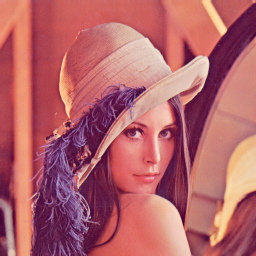
\includegraphics[width = 0.2 \linewidth]{ref.png}}
    \quad
    \centering
    \subfloat[Target]{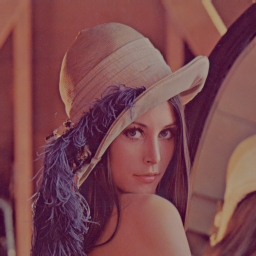
\includegraphics[width = 0.2 \linewidth]{tar.png}}
    \quad
    \centering
    \subfloat[Result]{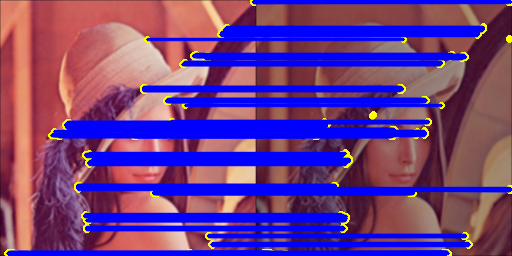
\includegraphics[width = 0.4 \linewidth]{R_sameEdge2_ref_to_tar.png}}
    \caption{주어진 이미지에 대한 edge detecting}
\label{fig:refImg}
\end{figure}

Figure~\ref{fig:refImg} 에서 ref. 이미지와 Target 이미지를 비교하여 보면, 이미지의 밝기가 다른것을 확인 수 있다. 이미지의 밝기는 Harris edge detecting을 적용하였을때, 민감도가 달라지는 결과를 초래한다. 이러한 경우에도 결과 이미지 Figure~\ref{fig:refImg} 을 보면, edge detecting되어 같은 엣지끼리 연결되는 것을 확인 할 수 있다.
\\또한, Figure~\ref{fig:refImg2}, \ref{fig:refImg3}에서 처럼 Shift와 약간의 회전이 가해진 Target과의 비교시에도 비교적 높은 확률의 정확도를 보여주었다.

\begin{figure}
    \centering
    \subfloat[Reference]{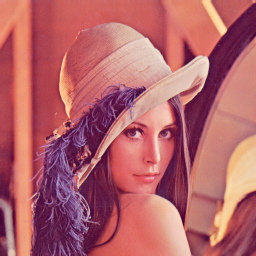
\includegraphics[width = 0.2 \linewidth]{ref.png}}
    \quad
    \centering
    \subfloat[Target (shifted)]{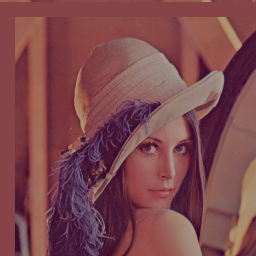
\includegraphics[width = 0.2 \linewidth]{tarShift.png}}
    \quad
    \centering
    \subfloat[Result]{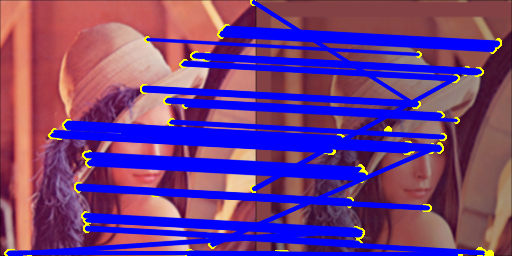
\includegraphics[width = 0.4 \linewidth]{R_sameEdge2_ref_to_shifted.png}}
    \caption{쉬프트된 이미지에 대한 edge detecting}
\label{fig:refImg2}
\end{figure}


\begin{figure}
    \centering
    \subfloat[Reference]{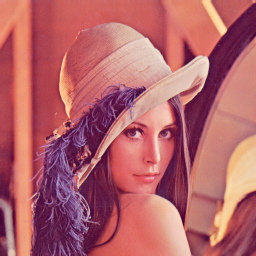
\includegraphics[width = 0.2 \linewidth]{ref.png}}
    \quad
    \centering
    \subfloat[Target (shifted)]{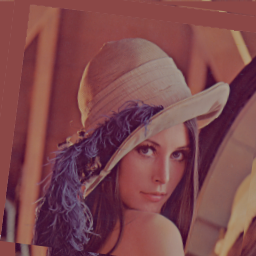
\includegraphics[width = 0.2 \linewidth]{tarShift_1.png}}
    \quad
    \centering
    \subfloat[Result]{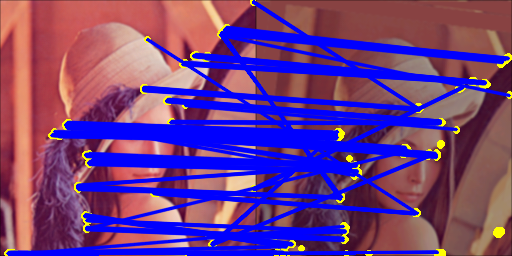
\includegraphics[width = 0.4 \linewidth]{R_sameEdge2.png}}
    \caption{쉬프트되고 회전된 이미지에 대한 edge detecting}
\label{fig:refImg3}
\end{figure}


\section{discussion}
이 과제의 경우, 소스 두개를 받아 각 소스의 웨이트를 비교하여야 한다. 기존의 main문에서 사용하는 방식으론 매우 코드가 복잡해질것이 뻔하니, setVision함수를 만들어 weight정보를 담고있는 pixel스트럭트를 반환하게 하였다. 또한 함수들과 상수들을 모두 헤더파일로 이동하였다. \\
기존 알고리즘에서 변경 한 부분이 있다. 먼저 Ref.와 Target 이미지는 서로 밝기 정보가 달라 Harris Edge detecting을 사용하면 같은 Threshold를 주었을때 서로 구해지는 엣지 갯수가 달라진다. 이를 해결하기 위해 Harris weight을 계산된뒤에 노말라이즈를 하였다. 결과적으로, 양쪽 모두 비슷한 엣지를 검출하게 되었다. 다만 노말라이즈를 사용하면 이미지의 밝기가 달라진경우엔 쉽게 대응할 수 있지만 대비가 달라진경우에 적절히 대응하지 못한다. 따라서 개선방법으로는 threshold를 사용자가 지정하는게 아니라 검출할 edge 갯수를 지정하고, 프로그램 내부에서 해당 갯수만큼의 edge가 나오는 threshold를 찾아내어 적용 하는 방식이 있겠다.  \\ 
두번째로 HOG weight을 구하는 과정에서 기존 코드는 180도를 20도 간격으로 나누어 0~20도를 0, 20~40도를 1 하는식으로 분류하였는데, 이는 경계에 가까울수록 부정확한 결과를 초래한다. 해당 부분을 수정하여,  더 높은 정확도를 얻을수 있는 linear한 방식을 사용했다. 0에서 8까지로 양자화 하는것은 같지만, 구간이 아닌 0, 20, 40 등의 경계선을 양자화하고 경계선에 가까운 정도를 두어 양쪽 경계선에 영향을 주도록했다. 예를 들어 30도라면 20도와 40도의 절반이므로 HOG weight을 구할때 $0.5\times magnitude$를 1번과 2번 차원에 넣는다. 이는 회전된 이미지를 감지하는데 더 높은 정확도를 지닌다.\\
결과적으로 약하게 회전된 두 이미지 간의 edge를 확인하고 서로 같은엣지를 확인하는데 매우 높은 정확도를 얻어내었다.

\end{document}